\documentclass[aspectratio=169]{beamer}
\usepackage[utf8]{inputenc}
\usepackage{amsmath,amssymb}
\usepackage[ngerman]{babel}
\usepackage{datetime}
\showdowfalse
\usepackage{array}
\usepackage{tabularx}
% use Swiss-style quotation marks (like in French)
\usepackage[autostyle,german=swiss]{csquotes}
\usepackage{framed} % or, "mdframed"
\makeatletter
\let\th@plain\relax
\makeatother
\usepackage[framed]{ntheorem}
\theoremstyle{plain}
\newframedtheorem{framed-def}{Definition}

\definecolor{FHNWyellow}{RGB}{253,231,14}
\definecolor{titlegrey}{RGB}{158,158,158}
\definecolor{bodygrey}{RGB}{188,188,188}
\definecolor{pitchblack}{rgb}{0, 0, 0}
\setbeamercolor{frametitle}{bg=FHNWyellow, fg=pitchblack}
\setbeamercolor{headline}{bg=FHNWyellow, fg=pitchblack}
\setbeamercolor{titlelike}{fg=pitchblack}
\setbeamercolor{title}{fg=pitchblack}
\setbeamercolor{item}{fg=pitchblack}
\setbeamercolor{section in toc}{fg=pitchblack}
\setbeamercolor{block body example}{fg=pitchblack,bg=bodygrey}
\setbeamercolor{block title example}{fg=pitchblack,bg=titlegrey}
\setbeamertemplate{section in toc}[sections numbered]
\usetheme{default}
\usecolortheme{wolverine}

\usepackage{tikz}
\usetikzlibrary{arrows.meta}
\usetikzlibrary{decorations.text}
\usetikzlibrary{shapes}
\usetikzlibrary{fit}
\usetikzlibrary{positioning, calc}
\usetikzlibrary{intersections}
\usepackage{./include/tikz-uml}
\tikzumlset{fill class=white}

\usepackage[export]{adjustbox}
\usepackage{changepage}

\makeatletter

\usepackage{listings}
\usepackage{listingsutf8}
\usepackage{courier}
\usepackage{graphicx}
\usepackage{textcomp}
\usepackage{hyperref}
\lstset{inputencoding=utf8/latin1}
\lstset{basicstyle=\tiny\ttfamily,breaklines=true}

\title[wodss]{Google Docs Light}
\subtitle{Final Presentation WODSS}
\author[Oliver Fabel, Melvin Johner]{Oliver Fabel\\Melvin Johner}
\newdate{date}{30}{05}{2022}
\date{\displaydate{date}}
\institute[FHNW]{
  Hochschule für Technik\\
  Fachhochschule Nordwestschweiz
}

\def\tabularxcolumn#1{m{#1}}
\beamertemplatenavigationsymbolsempty
\setbeamertemplate{footline}{
  \begin{tabularx}{\textwidth}{XX}
    \insertframenumber\hfill &
    \hfill
\includegraphics[height=0.5cm]{media/fhnw_10mm.jpg}
  \end{tabularx}
}

\begin{document}

\lstdefinestyle{inlinefontsize}{
  basicstyle=\ttfamily\lst@ifdisplaystyle\scriptsize\fi
}
\lstset{style=inlinefontsize}

\begin{frame}
    \titlepage
    \thispagestyle{empty}
\end{frame}

\begin{frame}
    \frametitle{Inhaltsverzeichnis}
    \tableofcontents
\end{frame}

\section{Architektur}
\begin{frame}
    \frametitle{Architektur}
    \begin{minipage}{0.48\textwidth}
        \begin{itemize}
            \item Programmiersprache: TypeScript
            \item Store Framework: Yjs
            \item Frontend Technologie: Vue.js
            \item Backend: Node.js
            \item Datenbank: MongoDB
            \item Middleware: Mosquitto
            \item Protokolle: Websockets und MQTT
        \end{itemize}
    \end{minipage}
    \hfill
    \begin{minipage}{0.45\textwidth}
        \begin{figure}
            \centering
            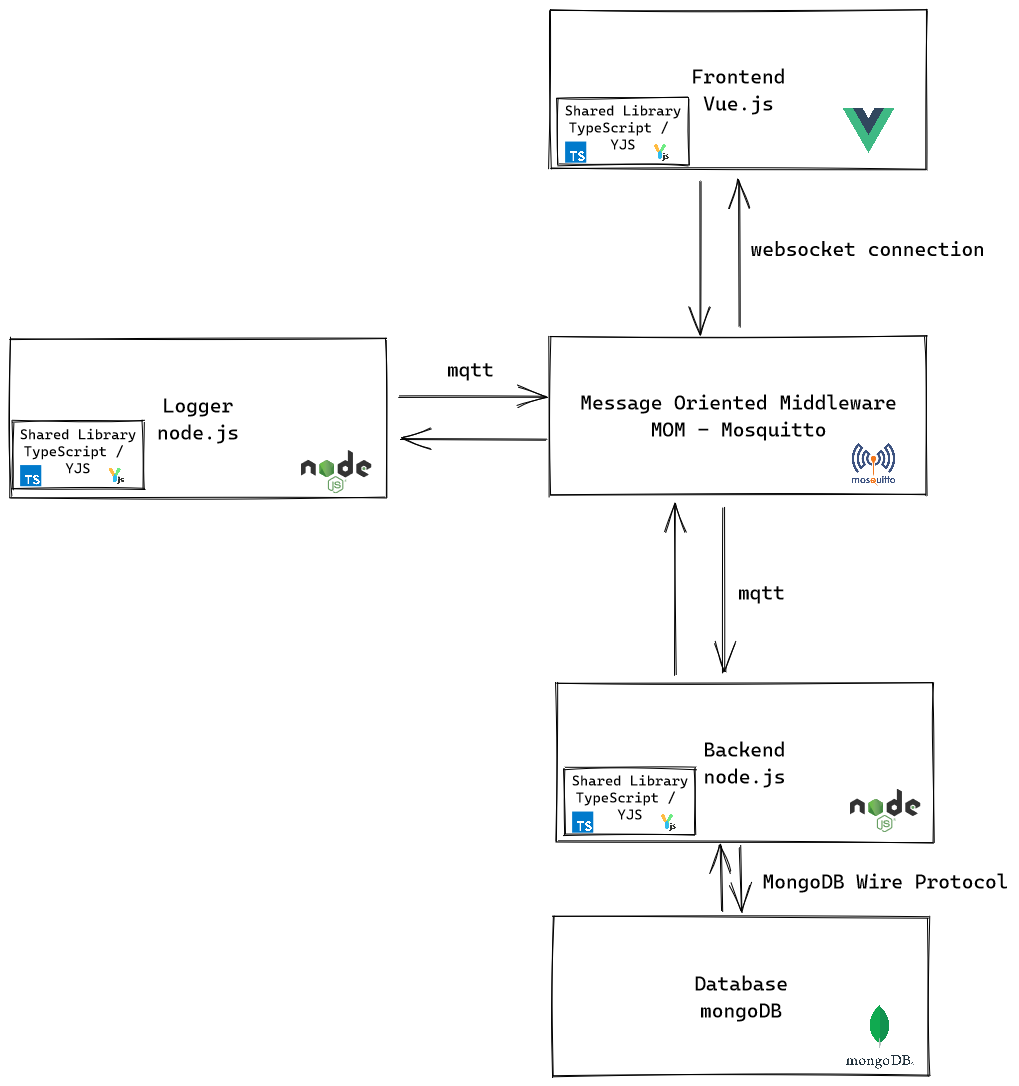
\includegraphics[height=6cm]{media/Big_Picture_wodss}
        \end{figure}
    \end{minipage}
\end{frame}
\begin{frame}
    \frametitle{Anpassungen seit der Midterm Präsentation}
    \begin{itemize}
        \item \textit{Synchronized Store} wurde vereinfacht: shadow und synchronized State wurden konsolidiert.
        \item Eine verteilte Mutex wurde implementiert.
        \item Eine synchronisierter Session Store wurde umgesetzt.
        \item Die Kommunikation über das Internet wurde mittels SSL abgesichert.
        \item Das Backend wurde hochverfügbar und gemacht.
        \item Eine externe Logging Komponente wurde umgesetzt.
        \item Persistierung des Document Store in einer MongoDB wurde eingerichtet.
    \end{itemize}
\end{frame}

\section{Bonus Features}
\begin{frame}
    \frametitle{Bonus Features}
    \begin{itemize}
        \item Hochverfügbares Backend
        \item Möglichkeit mehrere Dokumente parallel zu bearbeiten
        \item Chat pro Dokument
        \item Verteiltes Logging / verschiedene Logger
        \item Namengenerator à la Docker
        \item Farblich kodierte Benutzer
        \item Build Pipeline (CI/CD)
    \end{itemize}
    \begin{figure}
        \centering
        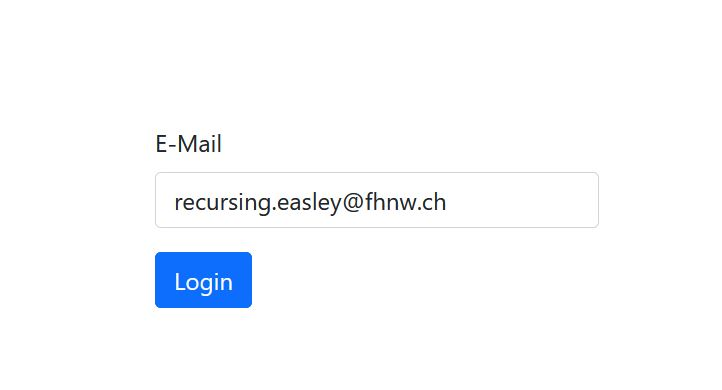
\includegraphics[height=4cm]{media/nameGenerator}
    \end{figure}
\end{frame}

\begin{frame}
    \frametitle{Hochverfügbares Backend}
    \begin{figure}
        \centering
        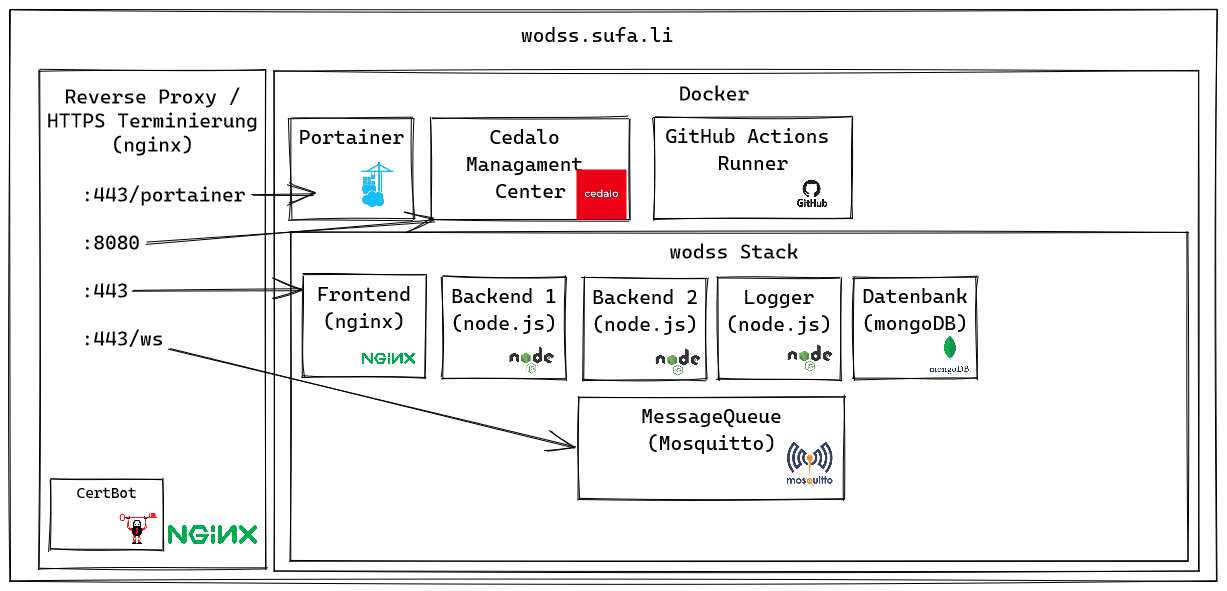
\includegraphics[height=6cm]{media/Physical_BigPicture_wodss}
    \end{figure}
\end{frame}
\begin{frame}
    \frametitle{Multi Document Edit}
    \begin{figure}
        \centering
        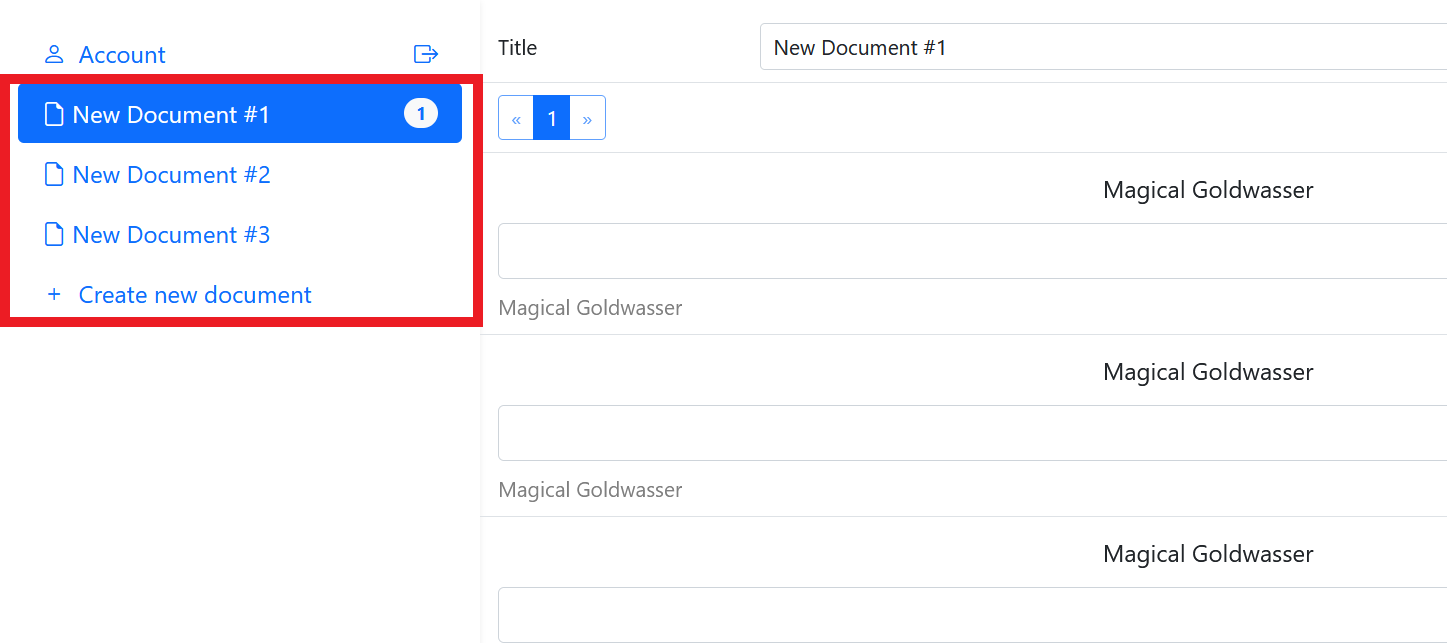
\includegraphics[height=6cm]{media/multiDocuemntEdit}
    \end{figure}
\end{frame}

\begin{frame}
    \frametitle{Chat pro Dokument}
    \begin{figure}
        \centering
        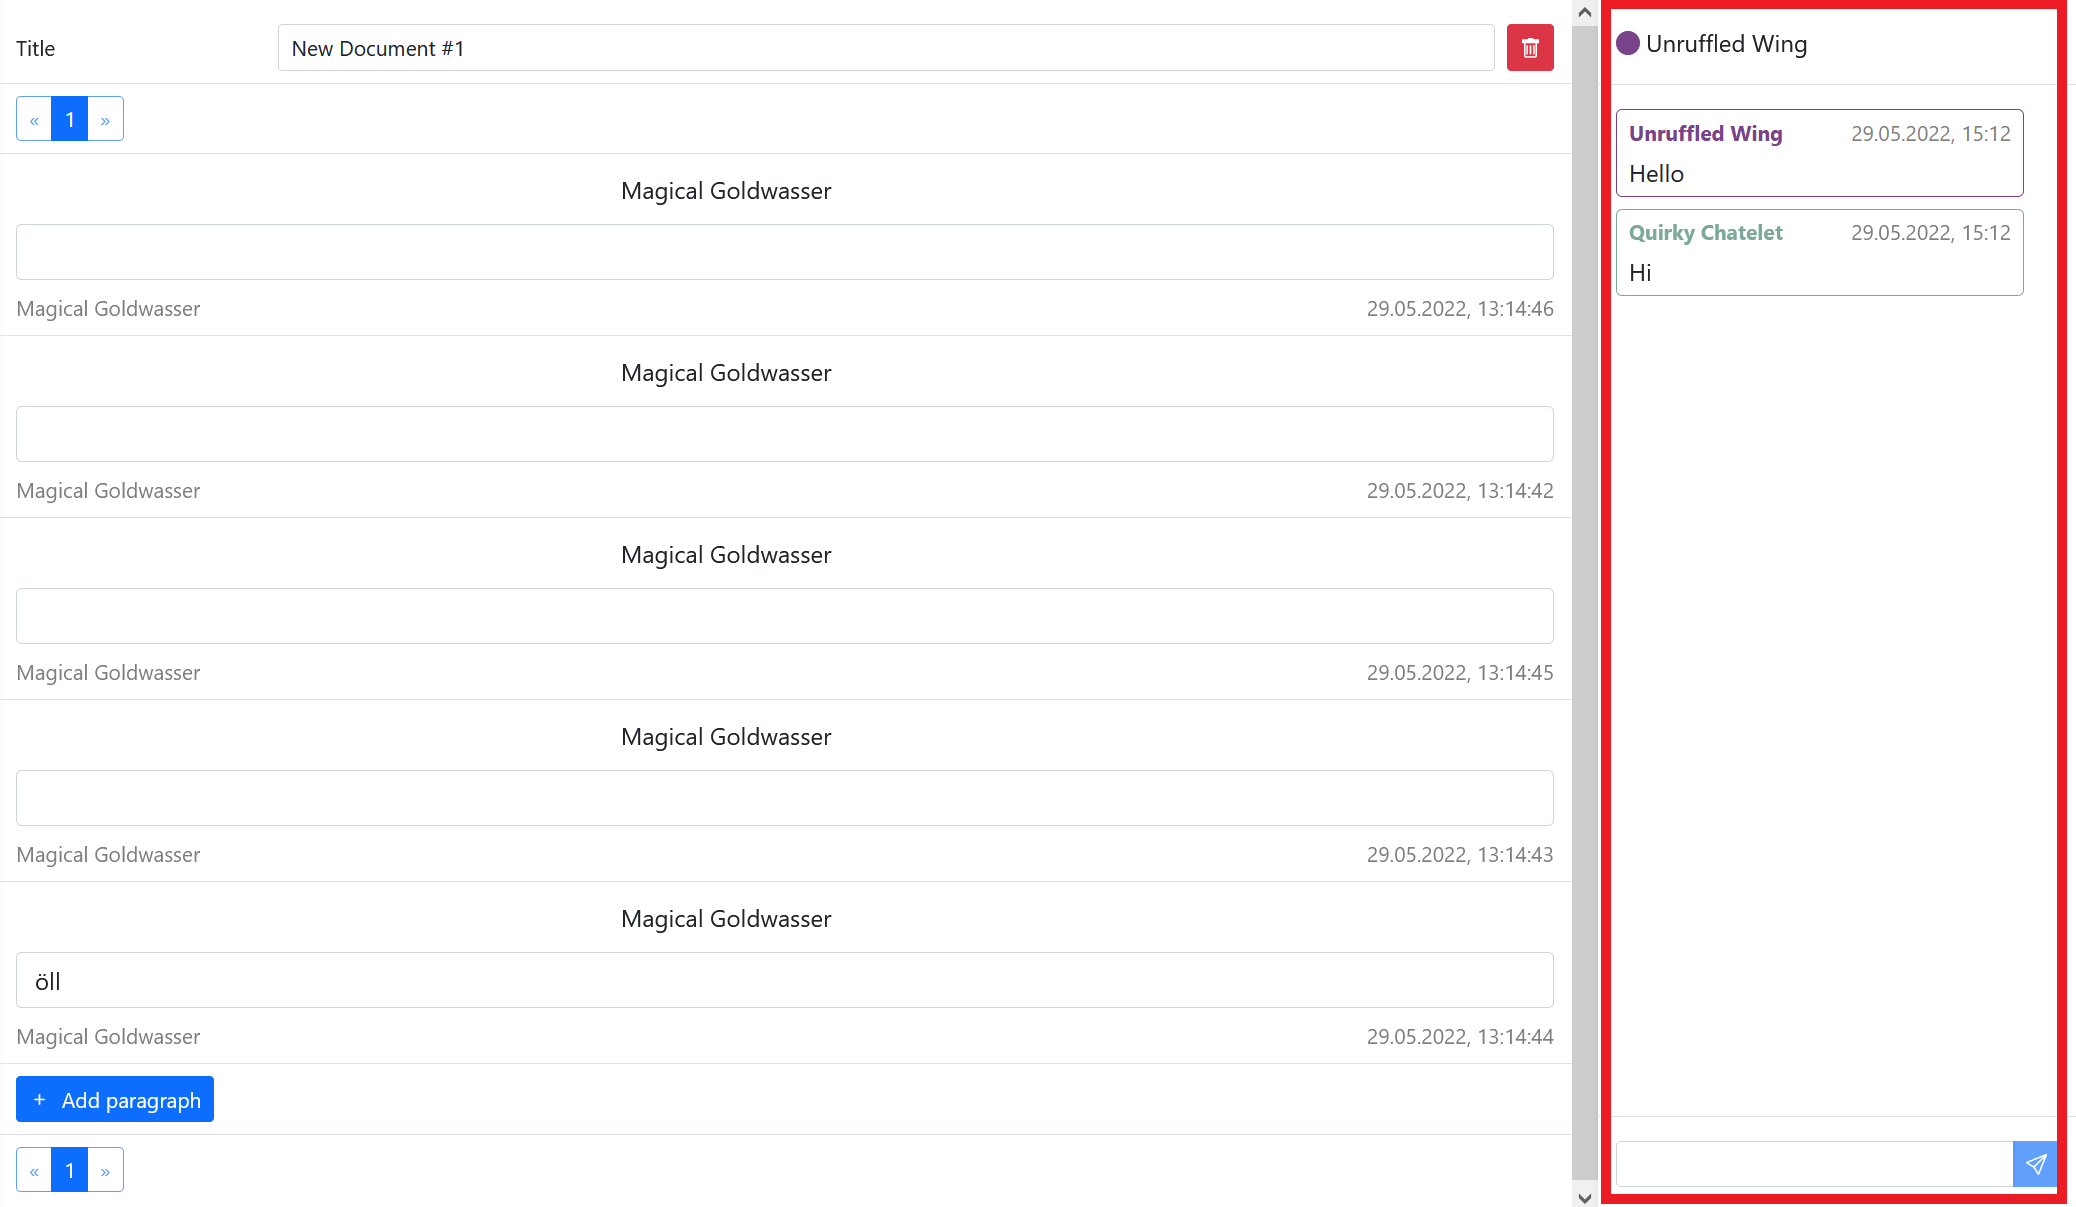
\includegraphics[height=6cm]{media/DocumentChat}
    \end{figure}
\end{frame}

%! Author = melvi
%! Date = 29/05/2022

\section{Review}
\begin{frame}
    \frametitle{Review und Erkenntnisse}
    \begin{itemize}
        \item Performance / E2E Testing gestaltete sich als schwierig
        \item Message Queues haben viel Potenzial
        \item Debugging in verteilten Systemen ist nicht immer einfach
        \item Typescript ist toll
        \item Vue.js hat seine Eigenheiten
    \end{itemize}
\end{frame}

\section{Ausblick}
\begin{frame}
    \frametitle{Ausblick}
    Mögliche Weiterentwicklungen:
    \begin{itemize}
        \item Dezentrale Validierung des verteilten Zustandes
        \item Offline Editierung von Dokumenten
        \item Monitoring mittels des \textit{Logging} Topics
        \item Benutzerverwaltung: Login und Berechtigungen
        \item Undo, Redo und Versionierung von Änderungen $\rightarrow$ volles Potential von Yjs nutzen
        \item Reduzierung der QoS auf 1
        \item Lastverteilung auf mehrere Backend Knoten
    \end{itemize}
\end{frame}


\section{Demo}
\begin{frame}
    \frametitle{Demo}
    \begin{center}
        \begin{figure}
            
\includegraphics[height=6cm]{media/qr-wodss-sufa-li.eps}
        \end{figure}
        \url{https://wodss.sufa.li/}\\
        \href{https://wodss.sufa.li/monitor.html\#eyJ1cmwiOiJ3c3M6Ly93b2Rzcy5zdWZhLmxpOjQ0My93cyIsInVzZXJuYW1lIjoibW9uaXRvciIsInBhc3N3b3JkIjoiUDRxckZpZXMwSEI5U1JkWnZURGl3bTZXWGN4SlVKczMifQ==}{Monitor}
    \end{center}
\end{frame}


\title{Vielen Dank für die Aufmerksamkeit}
\subtitle{Fragen?}
\author{}
\institute{}
\date{}
\begin{frame}
    \maketitle
    \thispagestyle{empty}
\end{frame}

\end{document}
